\documentclass[11pt,a4paper]{article}
\usepackage[margin=0.85in]{geometry}
\usepackage[T1]{fontenc}
\usepackage{lmodern,amsmath,booktabs,array,graphicx,longtable}
\usepackage{xurl}
\usepackage[hidelinks]{hyperref}
\usepackage{microtype}
\usepackage{fancyhdr}
\pagestyle{fancy}
\fancyhf{}
\fancyhead[L]{\small Digital access and circularity-related indicators}
\fancyhead[R]{\small Author review draft}
\fancyfoot[C]{\thepage}
\setlength{\headheight}{14pt}
\setlength{\parskip}{4pt}
\setlength{\parindent}{0pt}
\renewcommand{\arraystretch}{1.12}
\newcommand{\SampleN}{22}
\newcommand{\MainR}{0.779}
\newcommand{\MainRho}{0.810}
\newcommand{\MainP}{0.000020}
\newcommand{\PermutationP}{0.00005}
\newcommand{\BootstrapLow}{0.617}
\newcommand{\BootstrapHigh}{0.901}
\newcommand{\AdjustedP}{0.162}
\newcommand{\AdjustedBeta}{3.961}
\newcommand{\AdjustedLow}{-1.742}
\newcommand{\AdjustedHigh}{9.665}
\newcommand{\DigitalSDGRtwo}{0.658}
\newcommand{\DigitalEWasteRtwo}{0.292}
\newcommand{\DigitalSDGRMSE}{3.290}
\newcommand{\DigitalEWasteRMSE}{2.036}
\newcommand{\BaselineRtwo}{-0.098}
\newcommand{\XGBSDGRtwo}{0.555}
\newcommand{\XGBEWasteRtwo}{0.078}
\newcommand{\WithoutHaryanaR}{0.778}
\newcommand{\DeletionLow}{0.734}
\newcommand{\DeletionHigh}{0.819}
\newcommand{\EqualWeightR}{0.741}
\newcommand{\EWasteOnlyR}{0.365}
\newcommand{\EWasteOnlyP}{0.095}
\newcommand{\EWasteOnlyRho}{0.677}
\newcommand{\LogEWasteR}{0.642}
\newcommand{\SDGOnlyR}{0.802}

\title{Digital Access, Sustainability Indicators and Formal E-Waste Processing in Indian States}
\author{Yash Chauhan$^{*}$ \and Suresh Kumar Chelliah \and Shreya Srivastava}
\date{\small Department of Computational Intelligence\\
SRM Institute of Science \& Technology, Kattankulathur, Tamil Nadu, India\\[3pt]
\footnotesize yash.vks.chauhan@gmail.com; sureshkc@srmist.edu.in; ss1371@srmist.edu.in\\[3pt]
\footnotesize $^{*}$Corresponding author: Yash Chauhan\\[5pt]
\small Revised analysis: 26 October 2026}
\begin{document}
\maketitle
\begin{abstract}
Digital inclusion and circular economy policies can share an interest in information access and service coordination, but their association is sensitive to how development indicators are constructed. This study assembles seven traceable input tables for \SampleN{} Indian states, covering telecommunications, digital payments, income, sustainability, formal e-waste processing, and projected population characteristics. Digital access and a circularity-related proxy are constructed without a shared income component. We combine descriptive association, state resampling, income-adjusted regression, and nested cross-validation of separate sustainability and e-waste outcomes. The unadjusted index association is positive (Pearson $r=\MainR{}$, Spearman $\rho=\MainRho{}$), but the digital-access coefficient is uncertain after adjustment for log per-capita income (HC3 $p=\AdjustedP{}$). Digital-only ElasticNet achieves outer leave-one-state-out $R^2=\DigitalSDGRtwo{}$ for the SDG composite, compared with $\DigitalEWasteRtwo{}$ for log e-waste processing intensity. XGBoost does not outperform the regularized linear models. The pattern therefore supports a descriptive connection between digital access and broader development capacity, while providing more limited evidence for formal circular material processing. Mixed reference years, ecological measurement, rounded secondary UPI data, missing-state selection, and the small sample prevent causal or prospective forecasting claims. Policy use should distinguish broad sustainability indicators from direct evidence of circular activity.
\end{abstract}
\textbf{Keywords:} digital inclusion; circular economy; sustainability indicators; e-waste; Indian states; nested cross-validation.

\section{Introduction}
Digital connectivity can support information exchange, digital payments, and coordination across public and private services. These functions are potentially useful for waste collection, repair, reuse, and material recovery. The circular economy, however, is not interchangeable with broad economic or sustainability performance. Its measurement requires attention to resource loops and the activities through which materials remain in use \cite{geissdoerfer}.

This distinction matters in regional empirical research. A digitally connected state may also have higher income, a stronger administrative system, or more formal industrial activity. An association between a digital index and an environmental index can therefore reflect common development conditions. If income enters both indices directly, part of the relationship is built into their definitions. A transparent analysis must distinguish an observed association from mathematical overlap, confounding, and predictive performance.

This study examines that problem across Indian states. It uses tele-density and Unified Payments Interface (UPI) activity as broad indicators of digital access and use. Formal e-waste collected and processed provides a narrower administrative measure of material-processing activity, while the SDG India Index composite supplies a wider development benchmark. The study asks: (i) how strongly digital access is associated with an explicitly defined circularity-related proxy; (ii) whether the association persists after income adjustment and changes of specification; and (iii) whether digital indicators predict the two underlying outcomes equally well in held-out states.

The contribution is a reproducible state comparison with separate outcome validation. It is not a claim to invent the Digital Circularity Index name or to identify a causal effect of digital inclusion. Giraldi, Rossi, and Olivieri already develop a Digital Circularity Index for 14 Italian metropolitan cities using platform-adoption measures and partial least squares path modelling \cite{giraldi}. The present study instead examines broad access and payment indicators at Indian state scale and explicitly tests the gap between composite sustainability performance and formal e-waste activity.

\section{Conceptual framework}
Digital infrastructure may lower information and coordination costs, but general telephone subscriptions and payment transactions do not directly measure the use of repair or recycling platforms. Likewise, tonnes processed by registered facilities need not originate from the residents of the processing state. Material transfers, industrial concentration, and unrecorded informal processing can separate a state's processing footprint from its citizens' behavior.

Composite indicators help summarize heterogeneous measures but require explicit choices about normalization, weights, and interpretation \cite{oecd}. Here the combined proxy is a descriptive device. Its SDG component covers development beyond circularity, and its e-waste component covers one formal material stream. It should not be interpreted as an observed household behavior score or as a validated complete measure of a circular economy. Results for its components are therefore reported separately.

\section{Data and methods}
\subsection{Sources and sample construction}
Table~\ref{tab:sources} summarizes the seven analytical inputs. Source documents, extraction locators, and file hashes are retained in the accompanying reproducibility package. UPI values are secondary estimates published by Dataful using NPCI transaction data; they are not described as a directly obtained primary NPCI per-capita series. The public map reports whole-number values, which are used without invented precision \cite{dataful}.

\begin{table}[htbp]
\centering\small
\caption{Analytical inputs and reference periods.}\label{tab:sources}
\begin{tabular}{@{}>{\raggedright\arraybackslash}p{0.25\linewidth}>{\raggedright\arraybackslash}p{0.37\linewidth}>{\raggedright\arraybackslash}p{0.28\linewidth}@{}}
\toprule Input & Source / locator & Reference period \\
\midrule
Tele-density (subscriptions per 100 people) & TRAI, parliamentary reply via PIB, annexure \cite{trai} & 30 June 2024 \\
UPI transactions per person & Dataful article and state-map popups \cite{dataful} & FY2024--25 \\
Per-capita NSDP, current INR & Economic Survey, Table 1.11A \cite{nsdp} & FY2023--24; vintage 1 August 2025 \\
SDG composite (0--100) & NITI Aayog, state ranking \cite{sdg} & 2023--24 edition \\
Formal e-waste collected and processed, tonnes & MoEFCC/CPCB, PIB Annexure 1 \cite{cpcb} & FY2021--22 \\
Projected population & MoHFW Technical Group, Table 11 \cite{population} & 1 July 2021 \\
Projected urban share & Same report, Table 13 \cite{population} & 1 July 2021 \\
\bottomrule
\end{tabular}
\end{table}

All 28 states were considered; Union Territories were excluded for a consistent administrative comparison. Complete cases were retained without imputation. Arunachal Pradesh, Goa, Manipur, Meghalaya, Nagaland, and Uttar Pradesh had absent or dashed FY2021--22 e-waste entries in the cited source and were excluded. Missing entries were not coded as zero processing. The resulting sample contains \SampleN{} states. Inclusion is driven by recorded coverage, not representativeness of all Indian states.

The population denominator is a published projection, not a 2021 census enumeration. The ministry's 2020 population report was retrieved from a public mirror because the original URL was unavailable. PDF page and table references accompany the extracted values. Projected urban shares use the same date. Outdated literacy observations are not included in the revised models.

E-waste intensity is defined as tonnes collected and processed divided by projected population in millions, giving tonnes per million residents. The log outcome is $L_i=\log(1+E_i)$, where $E_i$ is this intensity. Income and population enter augmented models as natural logarithms. The sources span several years: the digital measures occur after the e-waste reference period. Prediction in this study is retrospective cross-state prediction, not a forecast or a test that later digital access caused earlier processing.

\subsection{Descriptive index construction}
For the observed cohort, each component is min--max normalized:
\begin{equation}
z_i(x)=100\frac{x_i-\min_j x_j}{\max_j x_j-\min_j x_j}.
\end{equation}
The digital access score $D_i$, circularity-related proxy $C_i$, and descriptive DCI are
\begin{align}
D_i &= \frac{4z_i(T)+3z_i(U)}{7},\\
C_i &= \frac{7z_i(E)+8z_i(S)}{15},\\
\mathrm{DCI}_i &= D_iC_i/100,
\end{align}
where $T$ is tele-density, $U$ is UPI transactions/person, $E$ is e-waste intensity, and $S$ is the SDG composite. These weights retain the relative non-income weights of the project's earlier specification after removing NSDP from both indices. They were documented before executing this revised analysis; they were not learned to maximize its correlations. The reanalysis is exploratory and was not preregistered.

All components now use the displayed normalization formula. The DCI has a sample-relative 0--100 scale. A zero indicates the cohort minimum under the chosen construction, not an absence of real digital access or environmental activity. DCI is used for descriptive comparison only. Predictive validation does not use a target constructed from full-sample extrema.

\subsection{Association, adjustment, and sensitivity}
We report Pearson and Spearman coefficients, a two-sided 19,999-permutation test, and a 10,000-resample state bootstrap percentile interval for Pearson correlation. These procedures treat states as exchangeable and do not resolve spatial dependence or selection. OLS models estimate the change per ten DAS points, with and without log NSDP as a covariate. Inference uses HC3 standard errors with t-based intervals. Additional specifications change component weights, remove Haryana, delete each state in turn, and isolate e-waste and SDG outcomes. These analyses are sensitivity checks, not independent confirmations. P-values are exploratory and not adjusted for a family of multiple comparisons.

\subsection{Nested predictive evaluation}
The predictive outcomes are $L_i$ and the original SDG composite, evaluated separately. The digital feature set has two variables: tele-density and UPI/person. The augmented set adds log NSDP, projected urban share, and log projected population. Ridge, ElasticNet, Random Forest, and XGBoost \cite{xgboost} are compared with small predefined parameter grids.

An outer leave-one-state-out loop produces one prediction for every state. Each outer training set uses shuffled four-fold inner cross-validation, seed 20261026, to select parameters by negative mean squared error. Scaling for the linear models is fitted inside the pipeline at every inner and outer training stage. Inner validation folds contain multiple observations, and no held-out outer state enters tuning. This separation addresses tuning optimism \cite{varma}; it does not remove limitations of a small, correlated ecological sample.

For observed outcomes $y_i$ and pooled outer predictions $\hat y_{-i}$,
\begin{equation}
R^2_{\mathrm{outer}}=1-\frac{\sum_i(y_i-\hat y_{-i})^2}{\sum_i(y_i-\bar y)^2}.
\end{equation}
RMSE and MAE are reported alongside an outer-training-mean baseline. $R^2$ is computed after pooling held-out predictions; it is not computed separately for one-observation LOO test folds. All inner scores, selected parameters, indices, and outer predictions are recorded. SHAP values \cite{shap} for XGBoost are calculated only for each outer model's held-out state; they explain the fitted prediction and are not causal effects.

\section{Results}
\subsection{Association and income adjustment}
Digital access and the combined proxy are positively associated: Pearson $r=\MainR{}$ ($p=\MainP{}$), Spearman $\rho=\MainRho{}$, permutation $p=\PermutationP{}$, with a state-bootstrap percentile interval of $[\BootstrapLow{},\BootstrapHigh{}]$. The association is descriptive; the broad SDG component is part of its interpretation. Figure~\ref{fig:association} contrasts the proxy and the direct processing outcome.

\begin{figure}[htbp]
\centering
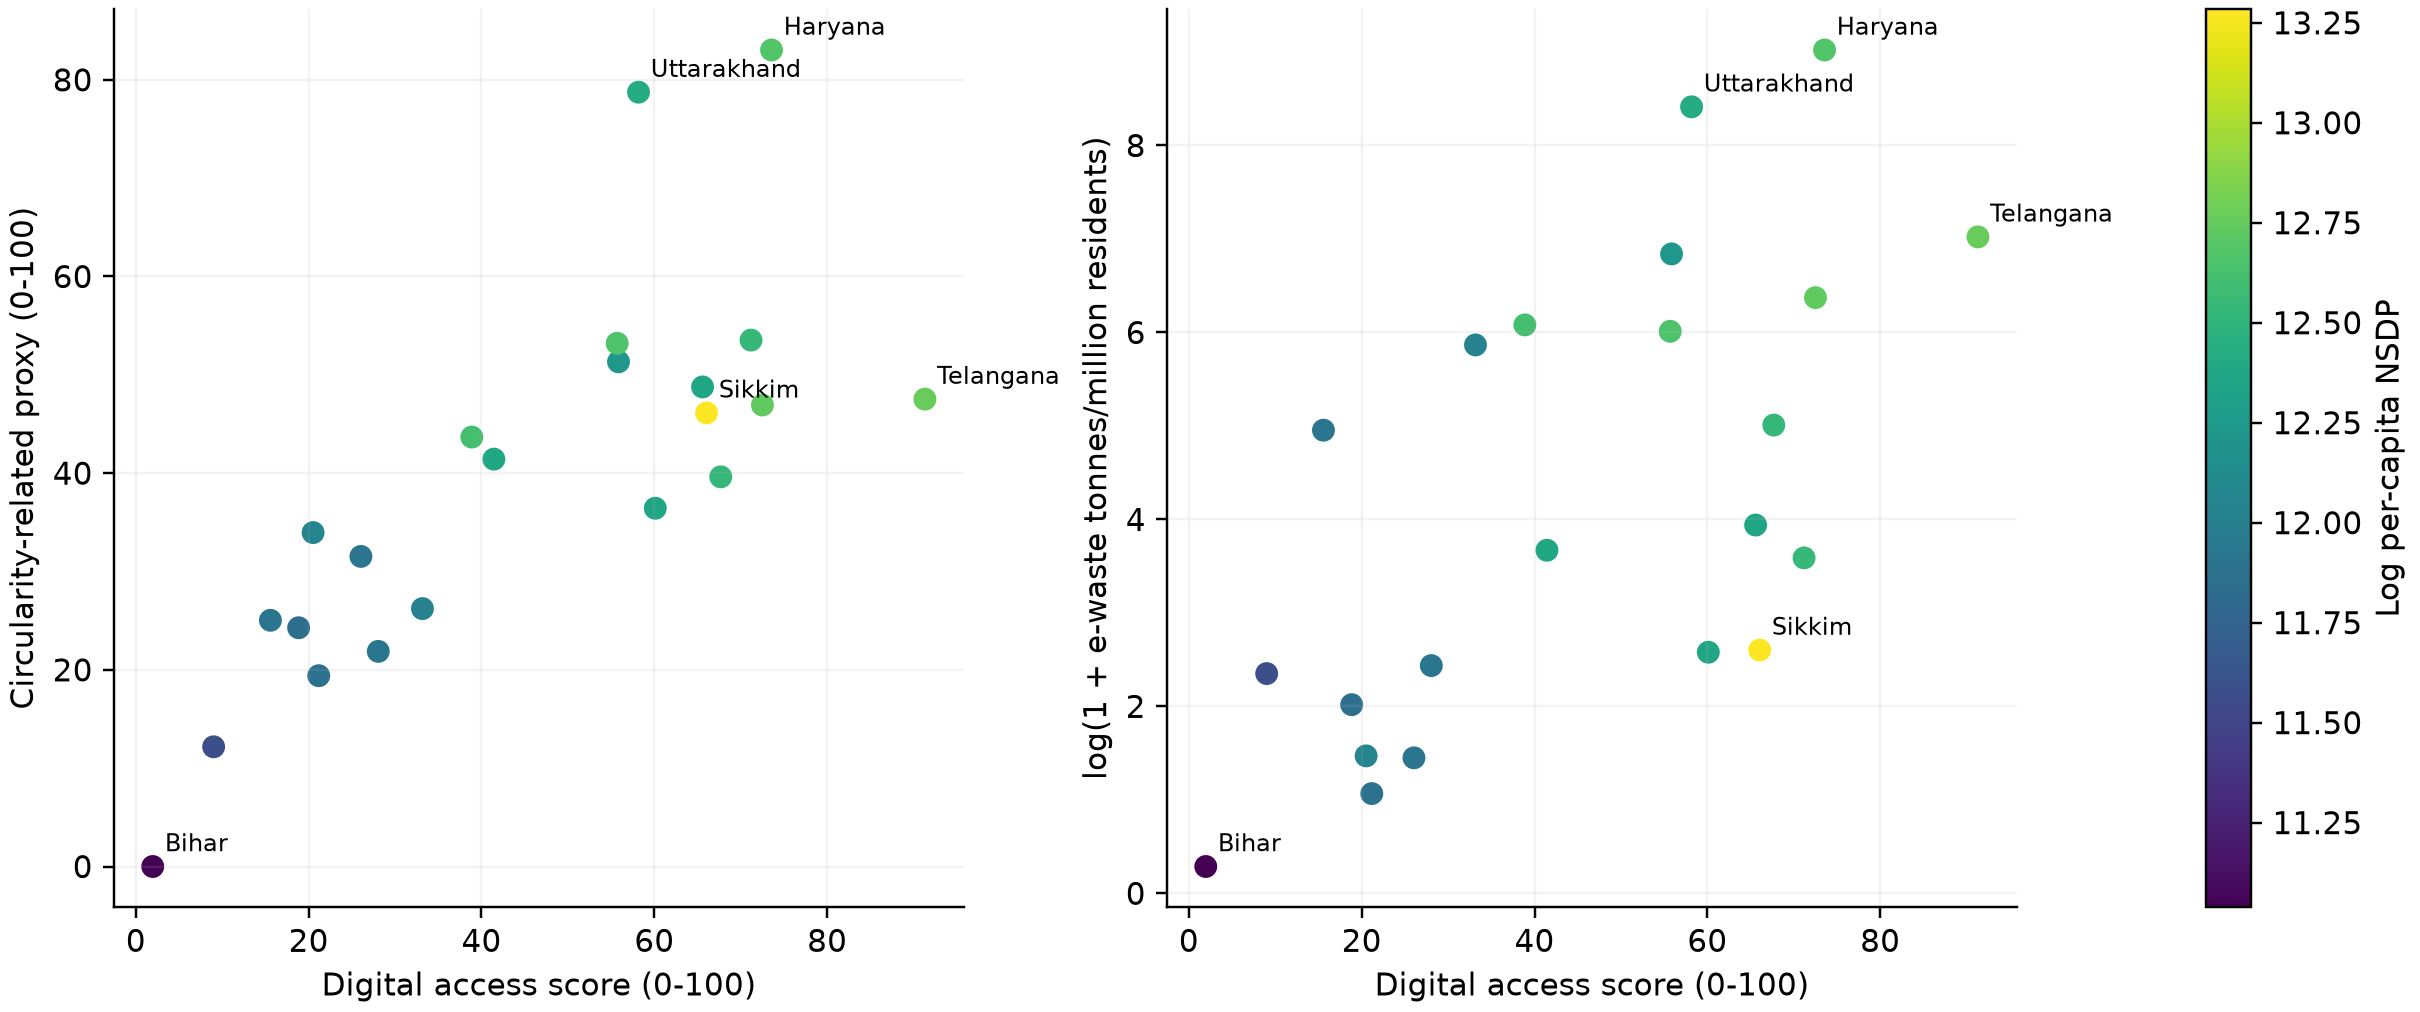
\includegraphics[width=\linewidth]{../figures/association.png}
\caption{Digital access against the combined proxy (left) and log formal e-waste intensity (right). Colour denotes log per-capita NSDP. Each point is a state; selected labels show influential or substantively relevant observations.}\label{fig:association}
\end{figure}

Table~\ref{tab:regression} shows why the association should not be interpreted as an independent digital effect. After log NSDP adjustment, the DAS coefficient for the proxy is \AdjustedBeta{} per ten points (95\% HC3 interval $[\AdjustedLow{},\AdjustedHigh{}]$, $p=\AdjustedP{}$). The estimate is imprecise and does not exclude zero. Income adjustment also leaves the digital coefficient uncertain for the separately analyzed e-waste and SDG outcomes. This does not prove there is no relationship; it limits claims about an independent association in this sample.

\begin{table}[htbp]\centering\small
\caption{DAS association per ten points, with HC3 standard errors and t-based inference.}\label{tab:regression}
\begin{tabular}{llrrr}\toprule Outcome & Log income control & Coefficient & 95\% interval & $p$ \\ \midrule
Combined proxy & No & 6.068 & [3.240, 8.896] & 0.0002 \\
Combined proxy & Yes & 3.961 & [-1.742, 9.665] & 0.1624 \\
Log e-waste intensity & No & 0.636 & [0.312, 0.960] & 0.0006 \\
Log e-waste intensity & Yes & 0.602 & [-0.423, 1.627] & 0.2341 \\
SDG composite & No & 1.847 & [0.950, 2.745] & 0.0004 \\
SDG composite & Yes & 0.686 & [-0.882, 2.254] & 0.3710 \\
\bottomrule\end{tabular}\end{table}


\subsection{Sensitivity and descriptive rankings}
Without Haryana, the Pearson association is \WithoutHaryanaR{}. Across all one-state deletions it ranges from \DeletionLow{} to \DeletionHigh{}. Equal component weights produce $r=\EqualWeightR{}$. The unlogged e-waste-only association is weaker ($r=\EWasteOnlyR{}$, $p=\EWasteOnlyP{}$); the rank association is \EWasteOnlyRho{}. For log e-waste intensity, Pearson $r=\LogEWasteR{}$. The DAS/SDG correlation is \SDGOnlyR{}. Thus the pattern depends on whether the outcome represents broad development, ranked processing activity, or its highly skewed magnitude.

Under this descriptive DCI, Haryana ranks highest, followed by Uttarakhand and Telangana. The rankings are not performance targets, efficiency scores, or population behavior estimates. Their meaning depends on the selected measures and reference cohort. The state-level table in Appendix~\ref{app:data} provides the corresponding values.

\subsection{Held-out prediction}
Table~\ref{tab:cv} reports every model/feature combination. Digital-only ElasticNet yields $R^2=\DigitalSDGRtwo{}$ for SDG scores and $R^2=\DigitalEWasteRtwo{}$ for log e-waste intensity. Their RMSE values are \DigitalSDGRMSE{} SDG points and \DigitalEWasteRMSE{} log units, respectively. The outer-training-mean baseline has $R^2=\BaselineRtwo{}$ for either outcome. Its negative value is retained rather than replacing it with a full-sample-mean benchmark that would use held-out information.

XGBoost's digital-only scores are \XGBSDGRtwo{} and \XGBEWasteRtwo{} for SDG and log e-waste, respectively. Its additional flexibility does not improve the observed outer predictions over the regularized linear alternatives. Augmented features do not consistently improve performance. The distinction between outcomes is more consequential than the use of a particular nonlinear algorithm. Comparisons across algorithms share the same states and should not be interpreted as independent replications or formal evidence of superiority.

\begin{table}[htbp]\centering\small
\caption{Pooled outer leave-one-state-out prediction scores. Inner tuning uses negative MSE.}\label{tab:cv}
\begin{tabular}{llrrrr}\toprule & & \multicolumn{2}{c}{Log e-waste} & \multicolumn{2}{c}{SDG composite} \\
Model & Features & $R^2$ & RMSE & $R^2$ & RMSE \\ \midrule
TrainingMean & none & -0.098 & 2.535 & -0.098 & 5.890 \\
Ridge & digital & 0.284 & 2.048 & 0.656 & 3.296 \\
ElasticNet & digital & 0.292 & 2.036 & 0.658 & 3.290 \\
RandomForest & digital & 0.105 & 2.289 & 0.606 & 3.527 \\
XGBoost & digital & 0.078 & 2.324 & 0.555 & 3.751 \\
Ridge & augmented & 0.269 & 2.069 & 0.605 & 3.534 \\
ElasticNet & augmented & 0.142 & 2.241 & 0.576 & 3.659 \\
RandomForest & augmented & 0.087 & 2.312 & 0.603 & 3.544 \\
XGBoost & augmented & 0.083 & 2.317 & 0.560 & 3.731 \\
\bottomrule\end{tabular}\end{table}


Held-out SHAP summaries for the augmented XGBoost models are included in the reproducibility package. They are conditional on a changing outer training model, a small correlated feature set, and the stated target. They are not used to establish that tele-density is a causal driver or that payments cannot be a mechanism.

\section{Discussion}
The strongest evidence is for co-occurrence of digital access and a broader sustainability/development benchmark. The formal processing result is less pronounced, sensitive to outcome scale, and uncertain once income is controlled. This suggests that a composite index can conceal important differences between development conditions and direct material-processing activity. A statistically strong descriptive index association is not sufficient evidence that digital infrastructure independently improves circular outcomes.

For policy, digital inclusion and environmental administration can be considered together when planning information systems, reporting, and access to public services. The present estimates do not identify the return to connectivity investment, establish a telecom threshold, or justify state funding allocations. Evaluation should use direct measures of collection, reuse, repair, formal and informal recycling, and material flows, with comparable periods and denominators.

The Indian-state comparison complements the metropolitan platform-focused DCI of Giraldi et al. \cite{giraldi}; the measures are not interchangeable. Broad telephone and payment metrics cannot validate the effects of particular circular platforms. The present work emphasizes transparent construction and outcome-specific checks rather than universal index novelty. This matters when transferring the idea to other regions: source compatibility and the meaning of the outcome should be reassessed before reusing weights or rankings.

\section{Limitations and future research}
First, only \SampleN{} states have complete reported inputs. Exclusion may depend on formal recycling activity and reporting capacity. Missing-state selection cannot be repaired by assuming zero values. Second, mixed reference periods and the timing of digital measures after e-waste activity prevent causal interpretation or prospective forecasting. Panel data aligned by year are needed.

Third, formal processing can include imported material and omit informal activity. It is not a waste-generation-adjusted recycling rate. The overall SDG composite contains many non-circularity dimensions and may conceptually overlap with digital development. Fourth, UPI estimates are rounded secondary values and omit unclassified state transactions. Tourism and business flows may affect transactions per resident. Tele-density counts subscriptions, not unique people with effective internet access.

Fifth, population and urban shares are projections from a 2020 report. They are consistently dated but remain uncertain estimates. Sixth, the sample supports only limited multivariable modeling. The regressions, bootstrap, permutations, and CV splits assume more exchangeability than may hold between neighboring or economically connected states. Spatially structured evaluation, external validation, and comparison with later administrative outcomes remain necessary. Finally, the reported analysis is exploratory, with several specifications and no preregistered primary endpoint. Model ranking and p-values should be interpreted accordingly.

\section{Conclusion}
Across \SampleN{} Indian states, digital access is positively associated with a descriptive circularity-related proxy. Income-adjusted estimates are uncertain, and predictive performance is considerably stronger for the broad SDG composite than for formal e-waste intensity. The findings support careful joint description of digital and sustainability conditions, while limiting claims about circular behavior, causal infrastructure effects, or AI-driven policy precision. The accompanying source records and nested evaluation provide a basis for subsequent analysis with richer, temporally aligned circularity data.

\section*{Data, code, and research statements}
The accompanying local reproducibility package contains the raw transcriptions, source locators and hashes, analysis specification, executable scripts, environment versions, state inclusion decisions, outer predictions, and tuning audits. Public deposition and any repository DOI remain pending author approval; no public repository is claimed. This study uses public aggregate state-level data without recruitment or individual records. This research received no external funding. The authors declare no conflicts of interest.

OpenAI Codex assisted source checking, Python implementation, and manuscript preparation. Numerical statements are linked to executable outputs; source and validation records accompany the draft. Human authors remain responsible for verifying the analysis, sources, authorship, and final submission text.

\textbf{Author contributions.} Yash Chauhan: conceptualization, methodology, software, validation, formal analysis, data curation, writing---original draft, writing---review and editing, and visualization. Suresh Kumar Chelliah: supervision. Shreya Srivastava: investigation and writing---review and editing. These roles and the author order were confirmed for this submission.

\begin{thebibliography}{99}
\bibitem{geissdoerfer} Geissdoerfer, M., Savaget, P., Bocken, N.M.P., and Hultink, E.J. (2017). The circular economy: A new sustainability paradigm? \textit{Journal of Cleaner Production}, 143, 757--768. \url{https://doi.org/10.1016/j.jclepro.2016.12.048}.
\bibitem{giraldi} Giraldi, L., Rossi, L., and Olivieri, M. (2026). Digital platforms and composite measurement of an urban circular economy: Developing the digital circularity index. \textit{Technology in Society}, 86, 103322. \url{https://doi.org/10.1016/j.techsoc.2026.103322}.
\bibitem{oecd} OECD/European Union/EC-JRC (2008). \textit{Handbook on Constructing Composite Indicators: Methodology and User Guide}. OECD Publishing. \url{https://doi.org/10.1787/9789264043466-en}.
\bibitem{dataful} Matta, A. (2026). Here is how UPI usage differs across Indian states. \textit{Dataful Insights}, 23 January. Article and state map, accessed 26 October 2026. \url{https://insights.dataful.in/articles/here-is-how-upi-usage-differs-across-indian-states}. Map: \url{https://flo.uri.sh/visualisation/27311082/embed}.
\bibitem{trai} Ministry of Communications (2024). Tele-density and Wi-Fi speed in the country. PIB, 19 December, PRID 2086009, Annexure; source TRAI Q2 2024 indicators. \url{https://www.pib.gov.in/Pressreleaseshare.aspx?PRID=2086009}.
\bibitem{nsdp} Ministry of Finance (2026). \textit{Economic Survey 2025-26, Statistical Appendix}, Table 1.11A, p. 32; data as on 1 August 2025. \url{https://indiabudget.gov.in/economicsurvey/doc/stat/tab1.11a.pdf}.
\bibitem{sdg} NITI Aayog (2024). \textit{SDG India Index 2023-24}. Overall state scores, reproduced in PIB release PRID 2032857, 12 July. \url{https://www.pib.gov.in/PressReleasePage.aspx?PRID=2032857}.
\bibitem{cpcb} Ministry of Environment, Forest and Climate Change (2024). Recycling of e-waste. PIB, 8 February, PRID 2004015, Annexure 1; CPCB data for FY2021-22. \url{https://www.pib.gov.in/Pressreleaseshare.aspx?PRID=2004015}.
\bibitem{population} National Commission on Population, Ministry of Health and Family Welfare (2020). \textit{Population Projections for India and States 2011-2036: Report of the Technical Group on Population Projections}, July; Tables 11 and 13. Archived copy: \url{https://educationforallinindia.com/wp-content/uploads/2023/04/Population-Projection-Report-2011-2036-upload_compressed_0-4.pdf}.
\bibitem{xgboost} Chen, T. and Guestrin, C. (2016). XGBoost: A scalable tree boosting system. \textit{Proceedings of ACM SIGKDD}, 785--794. \url{https://doi.org/10.1145/2939672.2939785}.
\bibitem{varma} Varma, S. and Simon, R. (2006). Bias in error estimation when using cross-validation for model selection. \textit{BMC Bioinformatics}, 7, 91. \url{https://doi.org/10.1186/1471-2105-7-91}.
\bibitem{shap} Lundberg, S.M. and Lee, S.-I. (2017). A unified approach to interpreting model predictions. \textit{Advances in Neural Information Processing Systems}, 30. \url{https://proceedings.neurips.cc/paper/7062-a-unified-approach-tointerpreting-model-predictions.pdf}.
\end{thebibliography}

\clearpage
\appendix
\section{State-level descriptive results}\label{app:data}
These scores use the revised \SampleN{}-state reference cohort. They should not be compared numerically with the old 16-state scores, which used different inputs, definitions, and normalization. E-waste is collected/processed tonnes per million projected residents; UPI values are rounded transactions/person.
\begin{longtable}{lrrrrr}
\caption{Revised cohort and descriptive indices.}\\
\toprule State & UPI/person & E-waste/million & DAS & Proxy & DCI \\ \midrule\endfirsthead
\toprule State & UPI/person & E-waste/million & DAS & Proxy & DCI \\ \midrule\endhead
Andhra Pradesh & 122 & 38.24 & 41.44 & 41.43 & 17.17 \\
Assam & 61 & 1.91 & 21.17 & 19.40 & 4.11 \\
Bihar & 44 & 0.33 & 1.96 & 0.00 & 0.00 \\
Chhattisgarh & 53 & 140.77 & 15.58 & 25.03 & 3.90 \\
Gujarat & 76 & 436.24 & 38.88 & 43.67 & 16.98 \\
Haryana & 136 & 8276.44 & 73.56 & 83.03 & 61.08 \\
Himachal Pradesh & 86 & 50.39 & 65.59 & 48.77 & 31.98 \\
Jharkhand & 50 & 9.49 & 9.01 & 12.17 & 1.10 \\
Karnataka & 203 & 584.46 & 72.51 & 46.93 & 34.03 \\
Kerala & 112 & 35.16 & 71.19 & 53.53 & 38.11 \\
Madhya Pradesh & 72 & 6.52 & 18.84 & 24.28 & 4.57 \\
Maharashtra & 185 & 148.76 & 67.69 & 39.62 & 26.82 \\
Mizoram & 77 & 12.18 & 60.12 & 36.43 & 21.90 \\
Odisha & 81 & 10.43 & 28.06 & 21.88 & 6.14 \\
Punjab & 72 & 933.27 & 55.86 & 51.32 & 28.67 \\
Rajasthan & 87 & 351.87 & 33.17 & 26.22 & 8.70 \\
Sikkim & 110 & 12.49 & 66.05 & 46.13 & 30.47 \\
Tamil Nadu & 107 & 407.21 & 55.70 & 53.20 & 29.64 \\
Telangana & 274 & 1119.85 & 91.31 & 47.52 & 43.40 \\
Tripura & 33 & 3.35 & 20.51 & 33.96 & 6.97 \\
Uttarakhand & 106 & 4505.74 & 58.17 & 78.74 & 45.81 \\
West Bengal & 51 & 3.26 & 26.05 & 31.53 & 8.21 \\
\bottomrule\end{longtable}

\end{document}
